% ****** Start of file aipsamp.tex ******
%
%   This file is part of the AIP files in the AIP distribution for REVTeX 4.
%   Version 4.1 of REVTeX, October 2009
%
%   Copyright (c) 2009 American Institute of Physics.
%
%   See the AIP README file for restrictions and more information.
%
% TeX'ing this file requires that you have AMS-LaTeX 2.0 installed
% as well as the rest of the prerequisites for REVTeX 4.1
%
% It also requires running BibTeX. The commands are as follows:
%
%  1)  latex  aipsamp
%  2)  bibtex aipsamp
%  3)  latex  aipsamp
%  4)  latex  aipsamp
%
% Use this file as a source of example code for your aip document.
% Use the file aiptemplate.tex as a template for your document.
\documentclass[%
 aip,
 jmp,
 amsmath,
 amssymb,
%preprint,%
 reprint,%
%author-year,%
%author-numerical,%
 numerical,
 longbibliography,
]{revtex4-1}

\usepackage{graphicx}% Include figure files
\graphicspath{{images/}}
\usepackage{dcolumn}% Align table columns on decimal point
\usepackage{bm}% bold math
\usepackage{url}
\usepackage{float}
\usepackage{silence}
\usepackage{tabularx}
\usepackage{verbatimbox}
\WarningFilter{revtex4-1}{Repair the float}
%\usepackage[mathlines]{lineno}% Enable numbering of text and display math
%\linenumbers\relax % Commence numbering lines

\begin{document}

%\preprint{AIP/123-QED}

\title[Laboratory 6]{Logic Gates} % Force line breaks with \\

\author{Kevin "Yama" Keyser}
 \email{kk8r8@mail.umck.edu}
\affiliation{ 
	University of Missouri-Kansas City
	%\\This line break forced with \textbackslash\textbackslash
}%

%\date{\today}% It is always \today, today,
             %  but any date may be explicitly specified

\begin{abstract}
In Laboratory 6, we cover logic gates and Boolean algebra. To accomplish this, we
use NAND and NOR gates with LEDs to show when values are true (high) or false (low).
\end{abstract}

%\keywords{Operational Amplifier}%Use showkeys class option if keyword
                              %display desired
\maketitle

%\begin{quotation}
%The ``lead paragraph'' is encapsulated with the \LaTeX\ 
%\verb+quotation+ environment and is formatted as a single paragraph before the first section heading. 
%(The \verb+quotation+ environment reverts to its usual meaning after the first sectioning command.) 
%Note that numbered references are allowed in the lead paragraph.
%
%The lead paragraph will only be found in an article being prepared for the journal \textit{Chaos}.
%\end{quotation}

\section{Background}

For this Lab, we need to know the basics of how Boolean Algebra works. You start off with 3 operators,
(AND represented by $\land$, OR represented by $\lor$, and NOT represented by $\neg$), and
using truth tables to figure out what the output would be.

The $\and$ is a binary operator (takes two inputs) and only puts out a true (high) value if both 
inputs are true (high). The truth table for an AND gate looks as follows

\addvbuffer[12pt 8pt]{
	\begin{tabularx}{0.45\textwidth}[t]{| X | X | X |}
	\hline
	\multicolumn{3}{|c|}{AND gate Truth Table}\\
	\hline
		\multicolumn{1}{|c|}{A} & 
		\multicolumn{1}{c|}{B} & 
		\multicolumn{1}{c|}{A$\land$B} \\ 
	\hline
	0 & 0 & 0 \\ \hline
	0 & 1 & 0 \\ \hline
	1 & 0 & 0 \\ \hline
	1 & 1 & 1 \\ \hline
	\end{tabularx}
}

The truth table takes all possible values of A and B, and lists them out, and what the corresponding output
would be. Whether you start off your values as false or true depends on your general outlook in life. Most
Computer Science classes will have you write the false values first (pessimists as they can be), and Philosophical
Logic classes will have you write the truth values first (blind optimists as they are). Since each variable can have
two separate values (0 and 1) in Boolean Algebra, you will have $2^n$ rows or possibilities.

Next, the $\lor$ gate is a binary operator that only puts out a false (low) value if both inputs are
false (low). The truth table for the OR gate looks as follows

\addvbuffer[12pt 8pt] {
	\begin{tabularx}{0.45\textwidth}[t]{| X | X | X |}
	\hline
	\multicolumn{3}{|c|}{OR gate Truth Table}\\
	\hline
		\multicolumn{1}{|c|}{A} & 
		\multicolumn{1}{c|}{B} & 
		\multicolumn{1}{c|}{A$\lor$B} \\ 
	\hline
	0 & 0 & 0 \\ \hline
	0 & 1 & 1 \\ \hline
	1 & 0 & 1 \\ \hline
	1 & 1 & 1 \\ \hline
	\end{tabularx}
}


Finally the $\neg$ gate. This is a unary operator (one input) and gives the inverse of what your
input was. As from Laboratory 5, you should notice that its symbol is similar to the Op Amps that
we used for our experiments. An Op Amp can be used as a NOT gate if you put your input through the
inverting pin, have your voltage supply for VCC+, but ground both the non-inverting, and VCC- pins.
The truth table for the NOT gate looks as follows

\addvbuffer[12pt 8pt] {
	\begin{tabularx}{0.45\textwidth}[t]{| X | X |}
	\hline
	\multicolumn{2}{|c|}{NOT gate Truth Table}\\
	\hline
		\multicolumn{1}{|c|}{A} & 
		\multicolumn{1}{c|}{$\neg$A} \\ 
	\hline
	0 & 1 \\ \hline
	1 & 0 \\ \hline
	\end{tabularx}
}

This is everything we need to be able to analyze any equation that uses Boolean algebra, which is what
our circuits that we are testing today use.

\section{Procedure}

The procedures for Laboratory 6 is very straight forward, so the Laboratory 6 sheet will be attached at the end of this write up.

\section{Presentation of Data}

	\subsection{6-1: Logic Levels}
	
	\addvbuffer[12pt 8pt] {
		\begin{tabularx}{0.45\textwidth}[t]{| X | X |}
		\hline
		\multicolumn{2}{|c|}{Voltage Cutoff Threshold for 7400}\\
		\hline
			\multicolumn{1}{|c|}{Bound} & 
			\multicolumn{1}{c|}{Voltage (V)} \\ 
		\hline
		Lower Bound & 0.650 \\ \hline
		Upper Bound & 1.21 \\ \hline
		\end{tabularx}
	}
	
	\addvbuffer[12pt 8pt] {
		\begin{tabularx}{0.45\textwidth}[t]{| X | X |}
		\hline
		\multicolumn{2}{|c|}{Frequency Cutoff for Stability}\\
		\hline
			\multicolumn{1}{|c|}{Wave Type} & 
			\multicolumn{1}{c|}{Frequency (MHz)} \\ 
		\hline
		Triangle & 2.3 \\ \hline
		Squre & 7.7 \\ \hline
		Sine & 3.4 \\ \hline
		\end{tabularx}
	}
	
	\begin{figure}[H]
	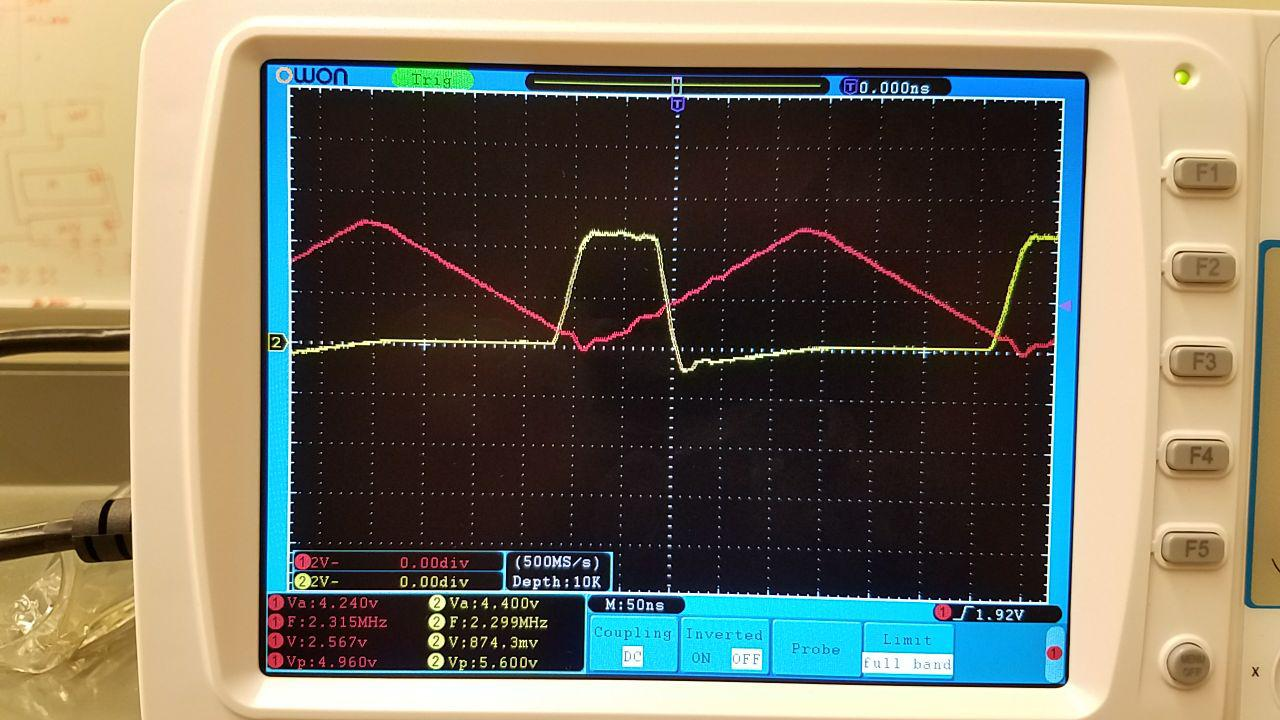
\includegraphics[width=\columnwidth]{Triangle.eps}
	\caption{Instability point for Triangle Wave.}
	\end{figure}
	
	\begin{figure}[H]
	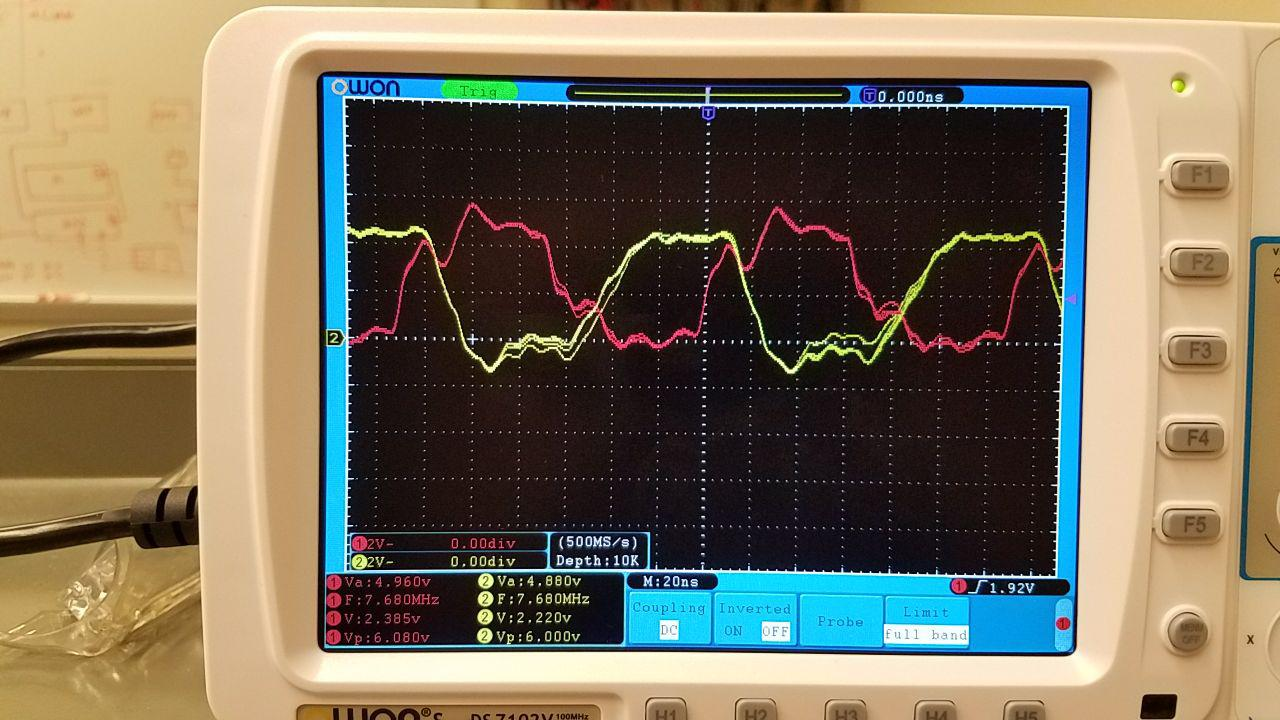
\includegraphics[width=\columnwidth]{Square.eps}
	\caption{Instability point for Square Wave.}
	\end{figure}
		
	\begin{figure}[H]
	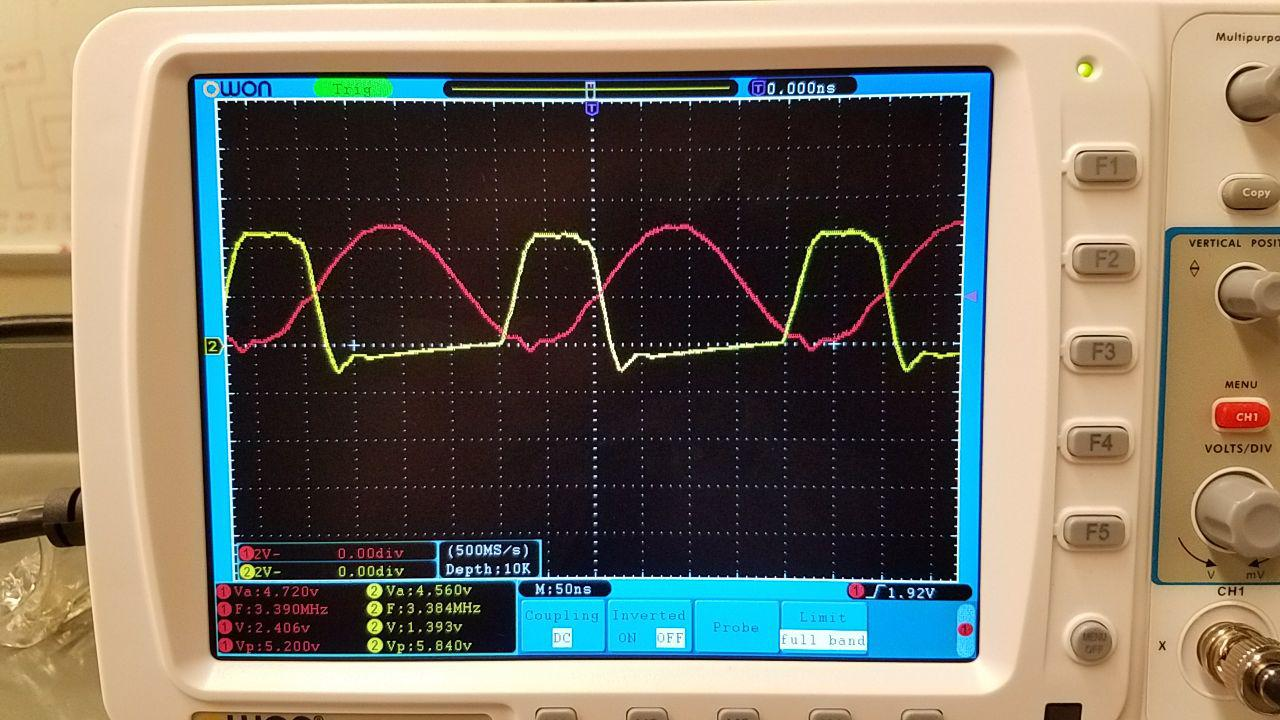
\includegraphics[width=\columnwidth]{Sine.eps}
	\caption{Instability point for Sine Wave.}
	\end{figure}		
	
	\subsection{6-2: NAND gates}
	
	\addvbuffer[12pt 8pt] {
		\begin{tabularx}{0.45\textwidth}[t]{| X | X | X |}
		\hline
		\multicolumn{3}{|c|}{NAND gate Truth Table}\\
		\hline
			\multicolumn{1}{|c|}{A} & 
			\multicolumn{1}{c|}{B} & 
			\multicolumn{1}{c|}{$\neg$(A$\land$B)} \\ 
		\hline
		0 & 0 & 1 \\ \hline
		0 & 1 & 1 \\ \hline
		1 & 0 & 1 \\ \hline
		1 & 1 & 0 \\ \hline
		\end{tabularx}
	}
	
	\addvbuffer[12pt 8pt] {
		\begin{tabularx}{0.45\textwidth}[t]{| X | X | X |}
		\hline
		\multicolumn{3}{|c|}{NOR gate Truth Table}\\
		\hline
			\multicolumn{1}{|c|}{A} & 
			\multicolumn{1}{c|}{B} & 
			\multicolumn{1}{c|}{$\neg$(A$\lor$B)} \\ 
		\hline
		0 & 0 & 1 \\ \hline
		0 & 1 & 0 \\ \hline
		1 & 0 & 0 \\ \hline
		1 & 1 & 0 \\ \hline
		\end{tabularx}
	}	
	
	\addvbuffer[12pt 8pt] {
		\begin{tabularx}{0.45\textwidth}[t]{| X | X | X | X | X |}
		\hline
		\multicolumn{5}{|c|}{4 input NAND Gate}\\
		\hline
			\multicolumn{1}{|c|}{A} & 
			\multicolumn{1}{c|}{B} & 
			\multicolumn{1}{c|}{C} & 
			\multicolumn{1}{c|}{D} & 
			\multicolumn{1}{c|}{$\neg$(A$\land$B$\land$C$\land$D)} \\ 
		\hline
		0 & 0 & 0 & 0 & 1\\ \hline
		0 & 0 & 0 & 1 & 1\\ \hline
		0 & 0 & 1 & 0 & 1\\ \hline
		0 & 0 & 1 & 1 & 1\\ \hline
		0 & 1 & 0 & 0 & 1\\ \hline
		0 & 1 & 0 & 1 & 1\\ \hline
		0 & 1 & 1 & 0 & 1\\ \hline
		0 & 1 & 1 & 1 & 1\\ \hline
		1 & 0 & 0 & 0 & 1\\ \hline
		1 & 0 & 0 & 1 & 1\\ \hline
		1 & 0 & 1 & 0 & 1\\ \hline
		1 & 0 & 1 & 1 & 1\\ \hline
		1 & 1 & 0 & 0 & 1\\ \hline
		1 & 1 & 0 & 1 & 1\\ \hline
		1 & 1 & 1 & 0 & 1\\ \hline
		1 & 1 & 1 & 1 & 0\\ \hline
		\end{tabularx}
	}	
	
\section{Discussion} \label{Section:Discussion}

	\subsection{6-1: Logic Levels}
	
	For the first part of this experiment, we used trial and error to figure out the 
	threshold for when the NAND gate went from a 1 (high) to a 0 (low). What we found
	was that any lower than 0.650V, and your input counted as a 0. Any higher than 1.21V
	and your input counted as a 1. This in-between area, inside the high and low threshold
	gave us inaccurate readings that fluctuated repeatedly. This may be due to tolerances,
	sensitivity, and the design of the gate to mainly have pulse or square waves as its input.
	
	The frequency dependency section, we raised the frequency of our function generator
	until the output signal no longer looked like a square wave. Looking at our table, you can
	see that the Square Wave had the most stability (up to 7.7 MHz) where the Triangle had the
	lowest (2.3 MHz), with the Sine Wave in between (3.4 MHz). When you look at the pictures,
	and consider how much time is spent in the the state of both being low, and that our window
	of stability from our previous experiment showed the voltage had to be below 0.650V, then the
	more time the input signal spends at the low state, the more stable our output signal will be.
	The square wave spends half of its time in the high state, and half of the time in the low state.
	Less so for the Sine Wave, and even less for the Triangle Wave. This means that the gate has
	less time to respond to changes, and the changes are more gradual, creating these inconsistencies
	and instabilities in our measurements.
	
	\subsection{6-2: NAND gates}
	
	What we get with our circuits with the LED is that it matches our truth table
	as we would expect. For the 2 input NAND and NOR gates, notice how they are just
	the opposite of the truth tables we had in the BACKGROUND section of our lab writeup.
	
	For the 4 input NAND gate (or even a 4 input AND gate) we could easily break down each
	into their own 2 input tables (A$\land$B, C$\land$D), and then combine their output
	into another 2 input gate. This is essentially what is happening on the inside
	(with oversimplifications due to higher level abstractions). You could also use
	De Morgan's Law, but that's outside the scope of this Lab.

\section{Conclusion}

This Lab was a very straight forward one, that will be expanded upon in the next Lab.
The biggest takeaway was the use of truth tables to solve Boolean Algebra problems.
There isn't an easier way to solve these as far as we know either (the 3-SAT problem
has been labeled an NP-complete problem in the field of Algorithm Analysis), so the
use of truth tables is the best we can do at this moment.

\end{document}